% !TeX spellcheck = en_GB
\chapter{Background}

\todo{Why do we want to see small things?}

Microscopy - imaging structures at microscopic scales - is an extremely wide and varied field. It is widely accepted to have began in the sixteen-hundreds, with Antoni van Leeuwenhoek's discovery of bacteria and other single-celled organisms \todo{ref}. After that, microscopes have been getting higher resolution, but as lenses got better and better, they were not the resolution bottleneck any more. Specifically, in 1873, Ernst Abbe determined that the best possible focus that a microscope can reach is limited by the wavelength of the light used \todo{ref}. This meant that the microscopes of the time were limited to a resolution of roughly 400 nm (assuming focused visible white light). It was long believed that the Abbe limit was a fundamental limit of nature, and that the only way around it was by using light of a different wavelength. This is one of the reasons for the development of electron microscopes \todo{ref}, as quantum mechanics postulates that accelerated electrons have much shorter wavelength than visible light. 

\todo{mention which books to read}

\section{Diffraction-limited fluorescence microscopy}

Fluorescence microscopy is an invaluable tool in modern biology \cite{Danial2016}. Unlike other methods, it is able to tag specific protein species and other relevant molecules in the cell with a fluorescent label. There are thousands of small organic fluorescent labels, and more are being developed \cite{Zhang2002, Resch-Genger2008}. The introduction of GFP and other fluorescent proteins was a remarkable development in the field, as labels can now be genetically fused to proteins of interest \cite{Shaner2005, Matlashov2020}. There were over thirty thousand papers collected in the PubMed database that mentioned fluorescence in the year 2020 alone. I will first explain the physical phenomena behind fluorescence, and then discuss why fluorescence microscopy is (or rather, used to be) limited by light diffraction.

\paragraph{Fluorescence.} In short, fluorescence is a phenomenon in which a molecule absorps a photon of one wavelength, spends a short amount of time in an excited energy state, and then emits a photon of another (longer) wavelength. The difference in wavelength is essential to perform microscopy, and the fact that molecules have discrete energy states is key to get there.

\begin{figure}
	\centering
	\includegraphics{jablonski diagram.ai}
	\caption{
		Illustration of the discrete energy states of a molecule and some possible transitions between them. The difference between energy levels determines the wavelength and colour of the absorbed or emitted photon.
	}
	\label{fig:jablonski}
\end{figure}

Let us consider a molecule with two electronic energy states, each of which has a number of vibrational energy levels as in \autoref{fig:jablonski}. When the molecule is in its ground state (the lowest available energy level), it can absorb photons only if the energy they carry matches the difference between the ground state and another energy level. From an excited state, the system can relax into lower vibrational levels without emitting radiation, after which it emits a photon, relaxing back to the ground state. Two possible paths are shown in the figure. Because some energy is lost in a non-radiative way, the emitted photons will carry less energy than the absorbed photon, resulting in the wavelength difference mentioned before. This is also called the Stokes shift. 

The precise energy levels available depend on the molecule and its environment. Therefore, every fluorescent molecule has a unique absorption and emission spectrum, which needs to be considered when planning a fluorescence experiment.

\paragraph{The diffraction limit.} We'll consider the diffraction limit in one of the simplest possible setups: an epifluorescence microscope. Epifluorescence microscopy is fairly similar to bright field microscopy. The sample, which is stained with a fluorescent dye, is illuminated with a laser at a wavelength that dye can absorb. The dye molecules will then emit photons of longer wavelengths in their emission spectrum, which are collected by the microscope objective. Before imaging by a CCD camera, the scattered laser light can be filtered away using a dichroic mirror that passes emission light and reflects excitation light. 

It used to be the case that microscopes were limited in resolution by the quality of their lenses and the pixel density of the CCD, but there is a much more fundamental limit, first described by Ernst Abbe. This limit is caused by the presence of an aperture. When a beam of light goes through an aperture of finite size, such as a lens, it cannot be focused onto an infinitesimal point. Instead, it will generate a spot with a radius approximately equal to $ \lambda/2\na $, where $ \lambda $ is the wavelength of the light and $ \na= n\sin\theta $ is the numerical aperture, the product of the index of refraction and the sine of the half-cone angle of the acceptance cone.

In particular, a circular aperture will convert point sources in the sample plane to Airy patterns in the image plane. Mathematically, this can be described by a convolution product between the point spread function (PSF) $ h $ and the object $ O $,
\begin{equation}
	I(\vb{x}) = (h * O)(\vb{x}) \coloneqq \int\dd{\vb{x}'} h(\vb{x}-\vb{x}')O(\vb{x}'),
	\label{eq:convolution}
\end{equation}
where the triple integration over the three components of $ \vb{x}' $ is implied, resulting in an image $ I $. When two fluorophores are close enough together that their PSFs overlap, they appear as a single object instead of two separate ones. This happens when the distance between them is around $ \lambda/2\na $, and that is what determines the resolution of a microscope. The exact resolution depends on your definition of this minimum resolvable distance. There are several definitions, but they are all proportional to $ \lambda/\na $. Some of them are listed in \autoref{tab:resolution limits} and visualised in \autoref{fig:diffraction limit}.

\begin{table}
	\centering
	\caption{Some common definitions of the resolution limit $ d_{xy} $.}
	\label{tab:resolution limits}
	\begin{tabularx}{\linewidth}{lXl}
		\toprule
		Name                              & Criterion                                                                               & Definition                   \\ \midrule
		Raileygh                          & The first minimum of one point's Airy function coincides with the maximum of another    & $ d_{xy} = .61\lambda/\na $  \\
		FWHM & The width of the Airy function at half of the peak height                               & $ d_{xy} = .51\lambda/\na $  \\
		Abbe                              & \todo{what did he base it on?}                                                          & $ d_{xy} = \phantom{1}.5\lambda/\na $   \\
		Sparrow                           & The distance between fluorophores at which the central maximum splits & $ d_{xy} = .47 \lambda/\na $ \\ \bottomrule
	\end{tabularx}
\end{table}

\begin{figure}
	\centering
	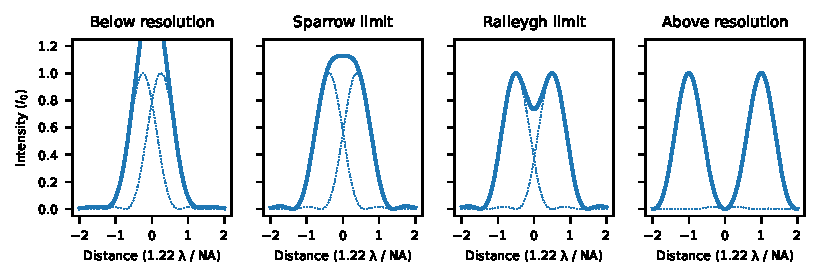
\includegraphics{diffraction_limit.pdf}
	\caption{Illustration of the diffraction limit.}
	\label{fig:diffraction limit}
\end{figure}

For a long time, physicists thought this limit was practically unavoidable \cite{McCutchen1967}, but in the next sections, I will discuss two ways in which one can get information from a system below the resolution limit. The first is indirect and requires playing with a new aspect of light (polarisation) that allows you to get information about structures that you cannot see. The second (STED microscopy) directly increases the image resolution. The excitation light is still subject to the Abbe limit, but we add another laser to effectively improve our focusing.

\section{Polarisation microscopy}

The wave nature of light might limit the resolution of a microscope, but it can also be exploited in our favour. Light polarisation can inform on the orientation of structures in a sample that are smaller than the diffraction limit. Among other things, this has been used to measure how the structure of DNA changes when it is subject to a strong stretching force, how integrin proteins respond to an applied force and measure the order of molecules embedded in the cell membrane, among others \cite{Backer2019, Nordenfelt2017, Swaminathan2017, Brasselet2013}. In this section, I will first introduce the concept of light polarisation, then discuss how it can be used in a microscope, and finally mention some optical components that affect the light polarisation, which are crucial to conducting a polarisation microscopy experiment.

\paragraph{The polarisation ellipse.} Remember that light is a transverse electromagnetic wave. This means that there are oscillations of the electric and magnetic fields along the path of a light ray, and that these oscillations are orthogonal to the propagation direction. In other words, if the light propagates along $\vb{k}$, the electric and magnetic fields $\vb{E}$ and $\vb{B}$ must satisfy $ \vb{E} \cdot \vb{k} = \vb{B} \cdot \vb{k} = 0$. (The fields themselves are also orthogonal to each other, so we can neglect $ \vb{B} $ without compromising our analysis.)

For the sake of simplicity, let's consider a ray propagating in the $ z $ direction. The electric field at any point in space and time can be written as
\begin{align}
	E_x(z, t) &= \Eox \cos(kz-\omega t + \phi_x),\\
	E_y(z, t) &= \Eoy \cos(kz-\omega t + \phi_y).
\end{align}
where $ \vb{E}_0 $ is the amplitude of the oscillation, $ k $ is the wavenumber (the length of $ \vb{k} $), $ \omega $ is the radial frequency and $ \phi $ is an arbitrary phase. Note that the wavenumber and the frequency are related to each other through the speed of light $ c $, since $ \omega = kc$. Note that the $ x $ and $ y $ components can have a phase difference.

Letting $ \delta = \phi_y-\phi_x $, it can be shown that 
\begin{equation}
	\left(\frac{E_x}{\Eox}\right)^2 - 2\cos\delta\frac{E_x}{\Eox}\frac{E_y}{\Eoy} + \left(\frac{E_y}{\Eoy}\right)^2 = \sin^2\delta.
\end{equation}
This is the equation for an ellipse. That means that, at any point in time, the point $ (E_x, E_y) $ lies on the ellipse defined by the equation above, which is called the polarisation ellipse. The ellipse is characterised by $ \Eox $, $ \Eoy $ and $ \delta $. Together, these values determine whether the polarisation is linear, circular, or something in between. Refer to \autoref{tab:polarisation states} for an overview.
\begin{table}
	\centering
	\caption{List of a number of polarisation states.}
	\label{tab:polarisation states}
	\begin{tabular}{lllll}
		\toprule
		Polarisation state      & $ \Eox $ & $ \Eoy $ & $ \delta $ & Jones vector \\ \midrule
		Linear along $ x $      & 1            & 0            & any        & $ (1, 0) $   \\
		Linear along $ y $      & 0            & 1            & any        & $ (0, 1) $   \\
		Linear at \ang{45}      & 1            & 1            & 0          & $ (1, 1) $   \\
		Circular (left-handed)  & 1            & 1            & $ \pi/4 $  & $ (1, i) $   \\
		Circular (right-handed) & 1            & 1            & $ -\pi/4 $ & $ (1, -i) $  \\ \bottomrule
	\end{tabular}
\end{table}


In general, the polarisation ellipse can be defined by means of two angles: the orientation $ \psi $ and ellipticity $ \chi $, as shown in \autoref{fig:pol ellipse}. They can be calculated from $ \alpha = \arctan(\Eoy/\Eox) $ and the phase difference $ \delta $ using
\begin{align}
	\tan 2\psi &= \tan 2\alpha \cos \delta,\\
	\sin 2\chi &= \sin 2\alpha \sin \delta.
\end{align}

\begin{figure}
	\centering
	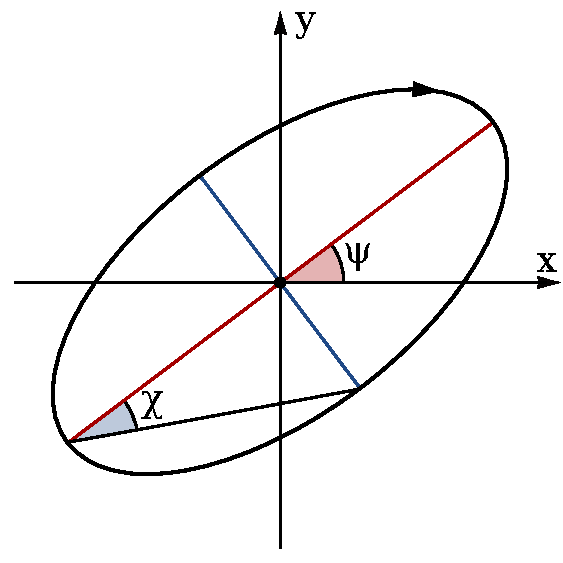
\includegraphics[width=.3\linewidth]{polarisation_ellipse.pdf}
	\caption{The meaning of $ \psi $ and $ \chi $ in the context of the polarisation ellipse. [by Wikipedia user Inductiveload]}
	\label{fig:pol ellipse}
\end{figure}

\paragraph{Microscopy.} Why is this relevant to microscopy? Well, since a fluorophore can be considered a small dipole moment, the absorption of excitation light that is linearly polarised along an angle $ \psi $ will depend on the dipole orientation $ \theta $. The intensity of light emitted by that fluorophore will then satisfy 
\begin{equation}
	\label{eq:malus}
	I(\psi, \theta) \propto \cos^2(\psi-\theta).
\end{equation}
This is Malus's law. Analogously, light emitted from a fluorophore is always linearly polarised parallel to its dipole. One can place a linearly polarising filter in front of the detector to measure a fluorophore's orientation. If the polariser emits light polarised at an angle $ \psi $, then the intensity measured at the detector also follows Malus's law, meaning that these two setups are analogous (not taking into account depolarisation effects in an experimental setup). As an example, see \todo{figure of sir actin from spira2017}.

\paragraph{Jones calculus.} To finish this section, I'd like to introduce Jones calculus. This is an incredibly useful way to model light polarisation, as well as how it interacts with certain optical components that are present in our system, but it does require us to express the the electric field with a complex function. Let us express it as follows:
\begin{equation}
	\vb{E}(z, t) = \vb{E}_0 e^{i(kz-\omega t)}.
	\label{eq:propagator}
\end{equation}
In the following analysis, we will treat $ \vb{E} $ as a two-dimensional vector with only an $ x $ and $ y $ component, as $ E_z = 0 $. Note that complex numbers are just a mathematical trick. The Maxwell equations that govern light propagation are linear, and taking the real part of a complex-valued function is also a linear operation, so the complex extension of $ \vb{E} $ will behave exactly the same as the actual electric field would. The phase difference between the two components is now contained in $ \vb{E}_0 $, which looks like
\begin{equation}
	\vb{E}_0 = \mqty(\Eox \\ \Eoy e^{i\delta} ).
\end{equation}
The Jones vectors for some special polarisation states are listed in \autoref{tab:polarisation states}.

The usefulness of Jones calculus lies in its ability to represent optical components as matrices acting on this vector. For example, a polariser that transmits $ x $-polarised light has the following matrix form:
\begin{equation}
	S_p = \mqty(1 & 0 \\ 0 & 0).
\end{equation}
It is easy to verify that $ S_p \vb{E}_0 = \Eox $. \todo{ref further along with rotated components to prove malus' law} We also need to take into account how mirrors affect polarisation. A mirror flips the field component that is orthogonal (the $ s $-component) to the mirror surface, while keeping the other component ($ p $) unchanged. So, a mirror whose surface is parallel to the $ x $-axis has a Jones matrix of the form
\begin{equation}
	S_{mx} = \mqty(1 & 0 \\ 0 & -1).
\end{equation}

Another important type of optical component in our setup is a waveplate. Waveplates or phase retarders are birefringent crystals, meaning the index of refraction a ray of light experiences is dependent on its polarisation. This happens when a crystal structure is not symmetric. \todo{what kind of symmetry?} In these crystals, \autoref{eq:propagator} is no longer valid and should be substituted by
\begin{equation}
	\vb{E}(z, t) = \mqty(\Eox e^{i(k_x z-\omega t)} \\ \Eoy e^{i(k_y z-\omega t + \delta)} ),
\end{equation}
assuming the optical axes of the waveplate are along $ x $ and $ y $. This can also be written as
\begin{equation}
	\vb{E}(z, t) = \mqty(\Eox  \\ \Eoy e^{i(\Gamma(z) + \delta)} ) e^{i(k_x z-\omega t)}
	\qq{, where}
	\Gamma(z) = (k_y-k_x) z.
\end{equation}
As one can see, a waveplate only imparts a delay on the $ y $-component of a beam, depending on its thickness $ z $ and its birefringence. We can neglect the common phase factor and represent the action of a waveplate by the following Jones matrix, 
\begin{equation}
	S_\Gamma = \mqty(1 & 0 \\ 0 & e^{i\Gamma}).
\end{equation}

Generally, waveplates are characterised by the relative delay they impart on the slowly propagating polarisation component. Quarter-wave plates delay it by a quarter of a wavelength compared to the fast propagating ray, corresponding to $ \Gamma = \pi/2 + 2n\pi $ (for any integer $ n $). Therefore, the Jones matrix of a quarter-wave plate satisfies 
\begin{equation}
	S_\qwp = \mqty(1 & 0 \\ 0 & i).
\end{equation}
Let's consider what happens to some specific cases. If vertically or horizontally polarised light passes through a quarter-wave plate, its polarisation will not change. But light polarised along $ +\ang{45} $ ($ -\ang{45} $) will be turned into left-handed (right-handed) light, and vice versa. Therefore, a quarter-wave plate allows us to convert between linearly and circularly polarised light. \todo{figure of waveplate actions}

The second type of waveplate we should treat is a half-wave plate. It features a delay of $ \Gamma = \pi + 2n\pi $, and its Jones matrix looks like
\begin{equation}
	S_\hwp = \mqty(1 & 0 \\ 0 & -1),
\end{equation}
which corresponds to mirroring the polarisation state along the $ x $-axis. Another way to think about that is that a ray polarised along an angle $ \psi $ will be rotated by an angle $ -2\psi $. Circularly polarised light will get the opposite handedness.

As said before, the power of Jones calculus lies in its ability to model the behaviour of a sequence of optical elements at arbitrary rotations. First, we need to define the Jones matrix for a rotated component. This is simply
\begin{equation}
	S(\theta) = R(\theta) \cdot S \cdot R(-\theta) 
	\qq{, where} 
	R(\theta) = \mqty(\cos\theta & -\sin\theta \\ \sin\theta & \cos\theta) \qq{\todo{check!}}
\end{equation}
and $ \theta $ is the angle of the component's $ x' $-axis with the lab coordinate system's $ x $-axis. \todo{introduce}. As an example, let's recover Malus's law by sending linearly polarised light through a half-waveplate at an angle $ \theta/2 $ (such that the light is polarised along $ \theta $ after it) and then through a polariser.
\begin{equation}
	I(\theta) \propto \abs{S_p(0) \cdot S_\hwp(\theta/2) \cdot \mqty(\admat{1 \\ 0})}^2 = \cos^2\theta.
\end{equation}

\todolist{
	\item Moeller calc	
	\item Hinting at psted
}

\section{Super-resolution microscopy}

There are several ways to glean information below the resolution limit. Some use optical properties of the sample to their advantage, like light polarisation or fluorescence resonance energy transfer (FRET) \cite{Lerner2021}, others use the photophysics of individual dyes to turn off a subset of them during imaging.  On the one hand, there are stochastic methods like STORM and PALM. On the other, there are targeted techniques such as STED, GSD, RESOLFT, ... \todo{explain acronyms} The Tegenfeldt group own a STED microscope. I will use this section to explain STED microscopy.

In essence, a STED microscope is a confocal microscope with an added laser that can selectively deplete fluorescence by stimulated emission.\todo{schematic of a sted microscope}  In a confocal microscope, the excitation laser does not illuminate the whole sample at once, but is scanned over it. This means only fluorophores in an Airy disk around the focus will be excited. Furthermore, the detector is now comprised of a pinhole and a photodetector (not a camera), which filters out most of the out-of-focus light. Therefore, the PSF of a confocal microscope is the product of the laser PSF $ h_\mathit{exc} $ and the detection probability $ h_\mathit{det} $
\begin{equation}
	h_\mathit{conf}(\vb{x}) = h_\mathit{exc}(\vb{x}) \cdot h_\mathit{det}(\vb{x}).
\end{equation}

Even though both of these PSFs are diffraction-limited, a STED microscope can reach an arbitrarily small resolution \cite{Wildanger2012}. It does so by illuminating the sample with a donut-shaped laser at a wavelength longer than the emission wavelength. Referring back to \autoref{fig:jablonski}, the blue laser excites the fluorophores that emit in green, but a red transition is also allowed. Under illumination with a red laser, this transition is made more favourable by the process of stimulated emission, first postulated by Einstein in 1926 \cite{Einstein1926}. This way, fluorophores at the edge of the excitation PSF can be prevented from emitting green light, while fluorophores at the centre do not experience stimulated emission, which reduces the width of the effective point spread function. An illustration of this effect is given in \todo{figure}.

Of course, the extent of the resolution improvement depends on the intensity of the depletion laser $ I_\mathit{dep}$. The STED resolution is
\begin{equation}
	d_\mathit{STED} = \frac{d_c}{\sqrt{1+d_c^2a^2\cfrac{I_\mathit{dep}}{I_\mathit{sat}}}},
\end{equation}
where $ d_c $ is the resolution limit of a confocal microscope, $ a $ the steepness of the donut pattern, and $ I_\mathit{sat} $ is the depletion intensity at which fluorophore brightness is reduced by half \cite{Harke2008}.
